\documentclass[tikz,border=6pt]{standalone}
% Shared visual language for the book's standalone vector figures.
% Keep this file compatible with the TeX Live version used by LyX.
\usepackage{amsmath,amssymb}
\usepackage{array,booktabs}
\usepackage{pgfplots}
\usepackage{pgfplotstable}
\usetikzlibrary{arrows.meta,calc,positioning}
\pgfplotsset{compat=1.17}

\definecolor{BookBlue}{HTML}{0072B2}
\definecolor{BookOrange}{HTML}{D55E00}
\definecolor{BookGreen}{HTML}{009E73}
\definecolor{BookGray}{HTML}{666666}
\definecolor{BookLightGray}{HTML}{D9D9D9}

\pgfplotsset{
  book axis/.style={
    axis line style={black!75,line width=0.55pt},
    tick style={black!75,line width=0.45pt},
    tick label style={font=\small},
    label style={font=\small},
    legend style={
      font=\small,
      draw=none,
      fill=none,
      cells={anchor=west},
    },
    grid style={BookLightGray,line width=0.35pt},
    major grid style={BookLightGray,line width=0.35pt},
  },
}

\begin{document}
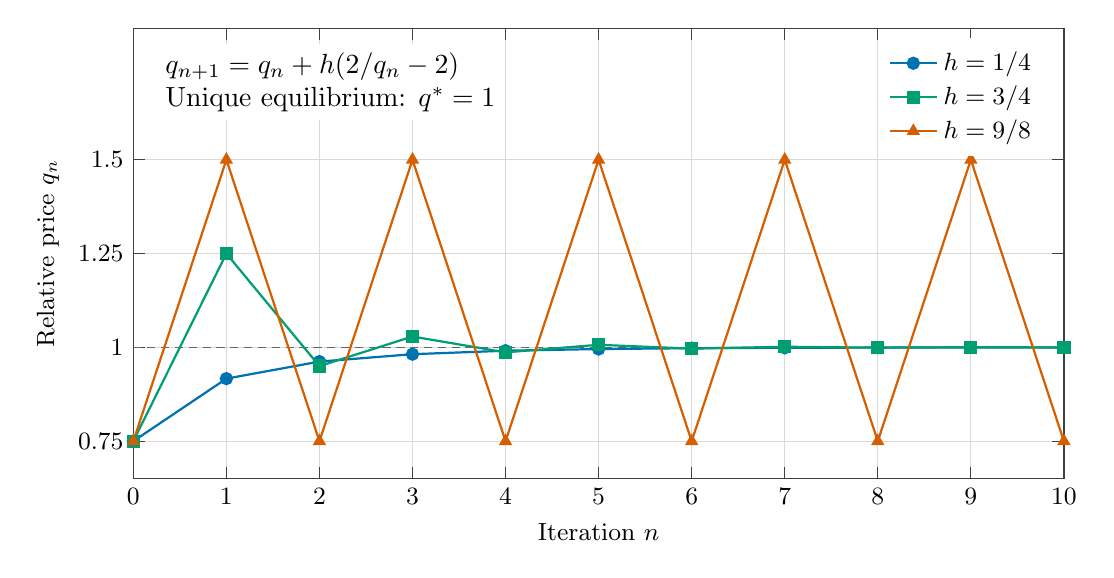
\begin{tikzpicture}
\begin{axis}[book axis,width=13.4cm,height=7.3cm,xmin=0,xmax=10,ymin=.65,ymax=1.85,
 xlabel={Iteration $n$},ylabel={Relative price $q_n$},xtick={0,1,...,10},
 ytick={.75,1,1.25,1.5},grid=major,
 legend style={at={(.98,.98)},anchor=north east,fill=white,
   fill opacity=1,text opacity=1,inner sep=3pt}]
 \addplot[BookGray,densely dashed,forget plot,domain=0:10]{1};
\addplot[BookBlue,thick,mark=*,mark size=2pt] coordinates{(0,0.750000000) (1,0.916666667) (2,0.962121212) (3,0.981806251) (4,0.991071699) (5,0.995576066) (6,0.997797862) (7,0.998901361) (8,0.999451285) (9,0.999725793) (10,0.999862934)};
\addlegendentry{$h=1/4$}
\addplot[BookGreen,thick,mark=square*,mark size=2pt] coordinates{(0,0.750000000) (1,1.250000000) (2,0.950000000) (3,1.028947368) (4,0.986747880) (5,1.006893026) (6,0.996624270) (7,1.001705016) (8,0.999151845) (9,1.000425157) (10,0.999787692)};
\addlegendentry{$h=3/4$}
\addplot[BookOrange,thick,mark=triangle*,mark size=2pt] coordinates{(0,0.750000000) (1,1.500000000) (2,0.750000000) (3,1.500000000) (4,0.750000000) (5,1.500000000) (6,0.750000000) (7,1.500000000) (8,0.750000000) (9,1.500000000) (10,0.750000000)};
\addlegendentry{$h=9/8$}
 \node[anchor=north west,fill=white,inner sep=3pt,align=left] at(axis cs:.25,1.81)
 {$q_{n+1}=q_n+h(2/q_n-2)$\\Unique equilibrium: $q^*=1$};
\end{axis}
\end{tikzpicture}
\end{document}
